\chapter{整体认知}

【摘要】本章回顾了人工智能的发展历史,并着重介绍了GLM系列模型。这些模型涵盖了语义理解、视频语义理解、图像生成、文本生成视频、图像生成视频、代码生成、智能代理(Agent)和多工具调用等多个领域。此外,讨论了大模型的思考与性能涌现,以及人工通用智能(AGI)的分级和未来的发展方向。

\section{引言}

自然语言处理(NLP)的发展历程中,算力从CPU到GPU的提升起到了关键作用,推动了模型从人工神经网络(ANN)向卷积神经网络(CNN)、循环神经网络(RNN)的演变,具体如下:

\begin{itemize}
	\item \textbf{算力提升历程}:早期NLP主要基于CPU计算,处理能力有限,难以应对大规模数据和复杂模型的训练需求。2000年代初,GPU开始被用于深度学习算法的加速。GPU具有强大的并行计算能力,能够同时处理大量数据,大大提高了深度学习模型的训练速度,使得训练更深层次、更复杂的神经网络成为可能。随后,NVIDIA、Google、Intel等公司开发了专门为深度学习设计的芯片,如NVIDIA的Tensor Core、Google的Tensor Processing Unit(TPU)等,进一步为NLP领域提供了高效的计算支持,推动了NLP技术的快速发展。
	\item \textbf{ANN阶段}:ANN是NLP早期应用的基础模型,它模拟人脑神经元之间的信息传递方式,由输入层、隐藏层和输出层组成,通过权重和激活函数来处理数据。早期的感知机就是一种简单的ANN,由Frank Rosenblatt在1958年提出,它开启了使用神经网络进行数据处理的时代,但只能处理线性可分问题。后来出现的多层感知机(MLP)在感知机基础上增加了隐藏层,并通过反向传播算法来训练,能够处理更复杂的非线性问题。不过,ANN在处理NLP任务时存在一些局限性,例如难以处理高维数据和序列数据,计算量较大且训练效率较低。
	\item \textbf{CNN阶段}:CNN是一类包含卷积计算且具有深度结构的前馈神经网络,具有表征学习能力。1989年,Yann LeCun提出了最早的卷积神经网络LeNet,用于图像分类,其包含卷积层和全连接层,规模远超此前的相关网络。1998年,LeCun及其合作者构建了更加完备的卷积神经网络LeNet-5,在手写数字识别中取得成功,定义了现代CNN的基本结构。2012年,AlexNet在ImageNet图像分类比赛中取得革命性成果,通过引入ReLU激活函数、Dropout正则化和GPU加速训练,显著提升了图像分类效果,标志着深度CNN成为计算机视觉领域的主流架构。此后,CNN也逐渐被应用于NLP领域,例如2013年Kim等人将CNN应用于文本分类任务,取得了较高的准确率。CNN通过卷积层和池化层可以自动提取文本的局部特征,减少了模型的参数量,提高了训练效率和泛化能力。
	\item \textbf{RNN阶段}:在处理文本等序列数据时,CNN难以捕捉数据的时间依赖性,而RNN引入了时间递归的结构,使得模型可以根据前一个时间步的状态输出当前步的预测,能够更好地处理序列信息,常用于机器翻译、文本生成等任务。但RNN容易在长序列中出现梯度消失问题,导致难以捕捉长距离依赖关系。为克服这一问题,LSTM(长短期记忆网络)应运而生,它通过引入记忆单元和门控机制,能够选择性地记住或遗忘信息,有效解决了长距离依赖问题,被广泛应用于NLP的各个领域。
\end{itemize}

在NLP向大模型演进的过程中,数据规模(data scale)的扩张与利用方式的革新是核心驱动力,从依赖大算力支撑到以大规模数据训练模型,经历了多个关键阶段,具体如下:

\subsection{从Transformer到BERT:数据规模与预训练范式的突破}

2017年,Google团队提出\textbf{Transformer模型},其基于自注意力机制(Self-Attention),摆脱了RNN的序列依赖限制,能够并行处理文本序列,为大规模数据训练提供了模型结构基础。Transformer的出现,让模型能够高效利用海量文本数据,突破了此前RNN在长序列处理和并行计算上的瓶颈。

2018年,Google基于Transformer推出\textbf{BERT(Bidirectional Encoder Representations from Transformers)},首次将“预训练+微调”范式推向成熟。BERT的预训练数据规模显著扩大,使用了BooksCorpus(约8亿词)和英文维基百科(约25亿词),总计超过30亿词的文本数据。  
\begin{itemize}
	\item 其核心创新是“双向预训练”,通过“掩码语言模型(MLM)”和“下一句预测(NSP)”任务,让模型从上下文双向学习文本语义,能够更全面地捕捉语言规律。  
	\item BERT的成功证明:当模型结构支持并行计算(依赖算力)且数据规模足够大时,预训练模型能在多种NLP任务(如文本分类、问答、命名实体识别)上超越传统方法,成为NLP领域的新基准。
\end{itemize}


\subsection{从BERT到GPT-1~2:数据利用率的跨越式提升}

与BERT同期,OpenAI团队聚焦“自回归语言模型”,推出了\textbf{GPT(Generative Pre-trained Transformer)} 系列,其数据利用方式与BERT形成鲜明对比:

\begin{itemize}
	\item \textbf{GPT-1(2018年)}:基于Transformer的解码器部分,采用“单向自回归预训练”(即通过前序文本预测下一个词),预训练数据包括BooksCorpus(约8亿词),与BERT初期数据规模接近。但GPT-1的核心目标是“生成式任务”,通过预训练后微调,在文本生成、摘要等任务上展现潜力。
	\item \textbf{GPT-2(2019年)}:数据规模和模型参数大幅提升——预训练数据扩展到“WebText”(从互联网爬取的约40GB文本,包含小说、博客、新闻等,总计约100亿词),模型参数从GPT-1的1.17亿增加到15亿。 更关键的是,GPT-2 通过 “零样本迁移” 能力颠覆了数据利用效率: 
        \begin{itemize}
            \item BERT的预训练任务(MLM)需要对输入文本进行“掩码”(随机遮盖部分词),实际参与训练的有效数据仅约15\%(被掩码的词);  
            \item 而GPT的自回归任务(预测下一个词)会利用输入的每一个词作为上下文,\textbf{数据利用率接近100\%}。这意味着在相同数据量下,GPT系列能更充分地学习语言模式,因此GPT-2在无微调的情况下,就能直接完成翻译、问答等多种任务,展现出“通用语言能力”的雏形。
        \end{itemize}
\end{itemize}

\subsection{从GPT-2到ChatGPT:数据对齐与“人类反馈”的融合}

2020年后,大模型的数据规模进一步爆炸(如GPT-3的预训练数据达45TB,包含万亿级词),但ChatGPT(2022年)的突破不仅依赖“更大数据”,更在于\textbf{数据利用方式的升级——引入“人类对齐数据”},让模型能力与人类需求匹配:

\begin{itemize}
	\item \textbf{基础:自回归预训练的延续}:GPT-3及后续模型(如GPT-3.5)仍以大规模互联网文本(书籍、网页、论文等)进行自回归预训练,通过预测下一个词学习通用语言规律,数据规模的扩张使其具备了更强的“知识储备”和“推理潜力”。
	\item \textbf{关键:标注数据驱动的对齐训练}:单纯的预训练数据(无标注的原始文本)只能让模型“懂语言”,但难以“懂人类意图”(如遵循指令、避免有害输出)。ChatGPT通过两步对齐机制解决这一问题:  
	\begin{itemize}
		\item \textbf{监督微调(SFT)}:收集人类标注的“高质量问答对”(如用户指令与理想回答),用这些数据微调预训练模型,让模型学会遵循具体指令;  
		\item \textbf{人类反馈强化学习(RLHF)}:让人类对模型的多个输出进行排序(标注“优劣”),再训练一个“奖励模型”,最后用强化学习(如PPO算法)让模型优化输出,使其更符合人类价值观(如友好、准确、安全)。  
	\end{itemize}
\end{itemize}

这些“标注数据”虽然规模远小于预训练数据(通常仅数万至数十万条),但针对性极强,相当于为模型提供了“人类行为准则”,最终让ChatGPT从“通用语言模型”升级为“能对话、可交互”的实用工具。


\subsection{总结:数据scale的核心逻辑}

从NLP到大模型,数据的演进不仅是“量的扩张”(从亿级到万亿级),更关键是“质的优化”:  

\begin{itemize}
	\item 早期依赖“无标注的大规模原始文本”,通过预训练让模型学习语言规律;  
	\item 后期通过“高质量标注数据”(如问答对、人类反馈),让模型从“学习语言”转向“理解人类需求”。  
\end{itemize}

而算力(如GPU集群、TPU)则是支撑这一过程的基础——没有足够的算力,既无法处理万亿级数据的预训练,也难以完成复杂的对齐训练。三者(算力、数据规模、数据利用方式)的协同,最终推动了大模型从实验室走向实际应用。

本书将重点介绍智谱AI(Zhipu AI)的相关模型,该公司成立于2019年。由清华大学计算机系知识工程实验室(KEG)技术成果转化而来,致力于打造认知智能大模型,专注于做大模型的中国创新。

2020年,智谱AI开始专注大模型算法研究。2021年9月,设计GLM算法,发布开源百亿大模型GLM-10B。2022年,合作研发了中英双语千亿级超大规模预训练模型GLM-130B,该模型是亚洲唯一入选斯坦福大学大模型中心评测的大模型,准确性、恶意性与GPT-3持平,鲁棒性和校准误差表现最佳。同年还发布了代码生成模型CodeGeeX和100+语言预训练模型mGLM-1B。

2023年,智谱AI推出千亿基座的对话模型ChatGLM及其单卡开源版本ChatGLM-6B,全球下载量超过800万。后续又发布了ChatGLM2、ChatGLM3等升级版本。2024年1月,推出新一代基座大模型GLM-4。2025年7月发布的GLM-4.5,在全球模型中排名第三,在国产模型和开源模型中均位居第一。

智谱AI在全球多地设有分研究中心,包括美国、英国、中东、新加坡等地。其在技术领域影响力较大,github排名总榜曾位居世界第五。

公司构建了丰富的产品矩阵,涵盖多种模态和功能,包括AI提效助手智谱清言、高效率代码模型CodeGeeX、多模态理解模型CogVLM、文生图模型CogView、文生视频模型CogVideo等。这些模型主要分为理解、创作/生成、安全、自动化执行等几个大方向,广泛应用于自然语言处理、计算机视觉等领域,为中国科协、华为、腾讯等1000余家企事业单位提供服务。


\section{GLM VS GPT}

智谱AI以自主研发的GLM(General Language Model,通用语言模型)框架为技术基底,逐步构建起覆盖多场景、多模态的系列大模型产品体系,其发展路径与技术定位对标OpenAI的GPT系列模型,如图\ref{fig:glmvsgpt}所示,具体体现为:

\begin{figure}[H]
	\centering
	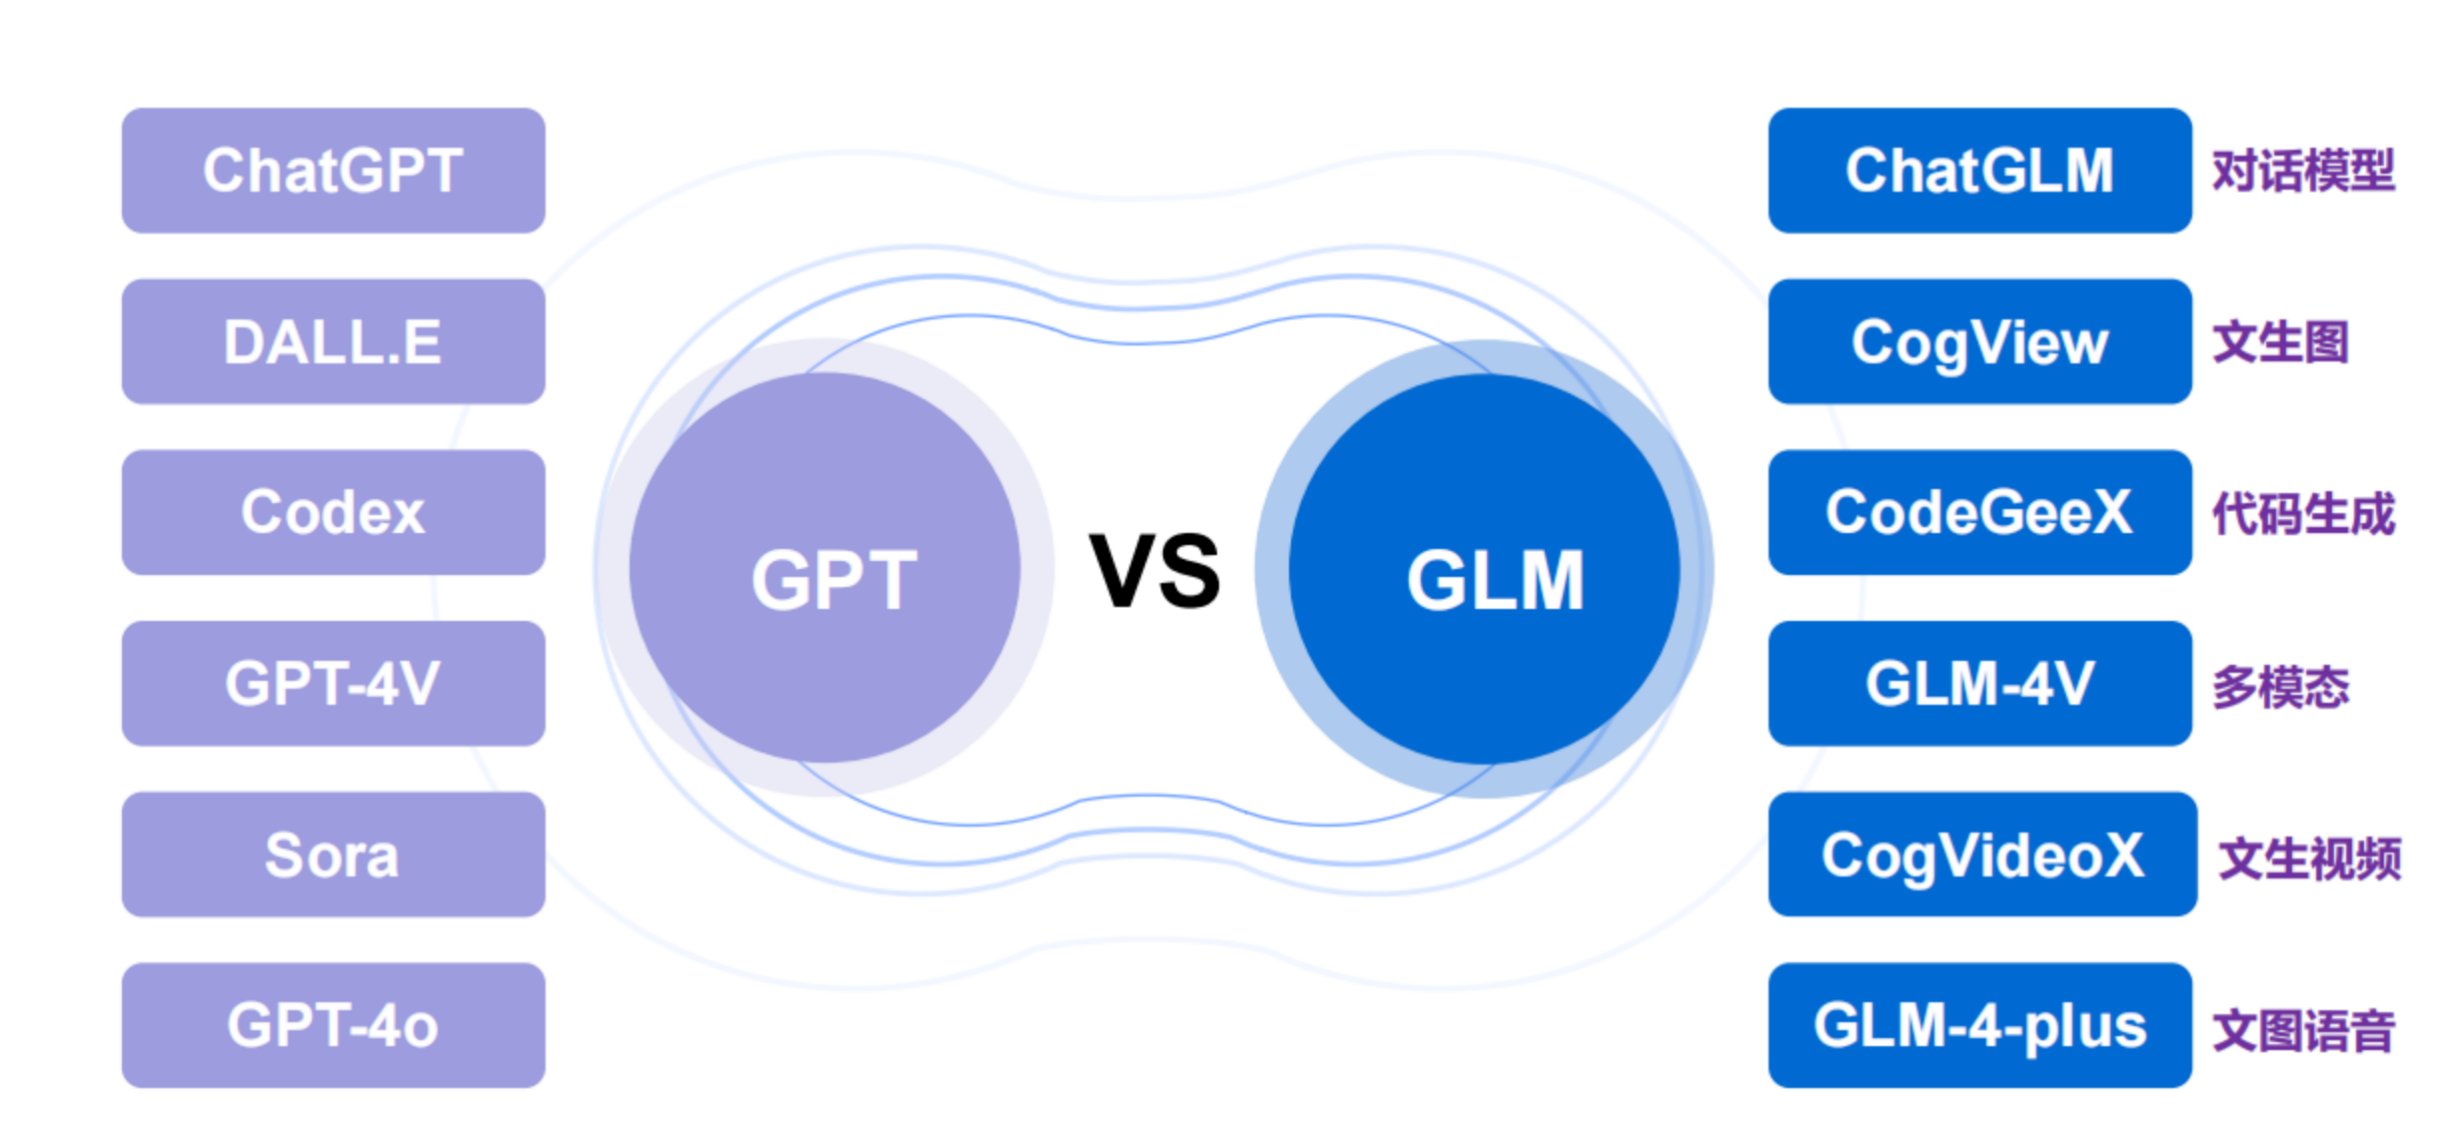
\includegraphics[width=0.8\textwidth]{figures/chapter1/fig1.png}
	\caption{GLM VS GPT}
	\label{fig:glmvsgpt}
\end{figure}

\begin{itemize}
	\item \textbf{核心框架的技术对标}:GLM框架采用双向注意力与自回归机制融合的创新架构,既具备类似GPT系列的长文本生成能力,又强化了对复杂语义的理解精度,在模型设计理念上与GPT的Transformer架构形成功能性呼应,为系列化模型开发奠定了统一技术基础。
	\item \textbf{产品迭代的路径对标}:从早期1300亿参数的GLM-130B(对标GPT-3),到对话优化的ChatGLM系列(对标ChatGPT),再到支持多模态交互的GLM-4及GLM-4.5(对标GPT-4),智谱AI的模型迭代既延续了GPT系列“参数规模扩张+能力边界拓展”的逻辑,又针对中文语境和垂直场景进行了深度优化,形成了与GPT系列在技术代际上的对应关系。
	\item \textbf{功能覆盖的场景对标}:如同GPT系列从文本生成向代码、图像、工具调用等领域延伸,智谱基于GLM框架推出的CodeGeeX(代码生成,对标GPT-4 Code)、CogVLM(多模态理解,对标GPT-4V)、Agent工具链(自动化执行,对标GPT-4的插件生态)等产品,构建了覆盖文本、代码、语音、图像、视频及智能执行的全栈能力,实现了与GPT系列在功能场景上的全面对标。
\end{itemize}

这种以GLM框架为核心的系列化布局,既体现了对国际前沿技术路线的对标跟进,也通过本土化技术创新形成了差异化竞争力,推动其成为国内大模型领域与OpenAI GPT系列具有直接可比性的技术体系。

2024 年 8 月,智谱 AI 在 KDD 国际数据挖掘与知识发现大会上发布了新一代基座大模型 GLM-4-Plus。该模型在多个指标上接近甚至超越了 GPT-4o, 如图\ref{fig:glm4plus}所示。

\begin{figure}[H]
	\centering
	\includegraphics[width=0.8\textwidth]{figures/chapter1/fig2.png}
	\caption{GLM-4-Plus与GPT-4o的中英文能力对比}
	\label{fig:glm4plus}
\end{figure}

GLM-4-Plus 在语言理解、指令遵循、长文本处理等方面性能得到全面提升。在各大语言文本能力数据集上,它获得了与 GPT-4o 及 405B 参数量的 Llama3.1 相当的水平。其通过更精准的长短文本数据混合策略,取得了更强的长文本推理效果,长文本能力比肩 GPT-4o,超过 Gemini 1.5 Pro 和 Claude Sonnet 3.5。

在与 GPT-4o 的全面较量中,GLM-4-Plus 已经可以在大多数任务上做到逼近,甚至在某些逻辑推理等任务上实现了超越。在最新的 SuperBench 大模型评测中,GLM-4-Plus 位列世界前三,打破了此前国外模型垄断前三甲的局面。


ChatGLM体现出较强的语义推理能力,如图\ref{fig:chatglm}所示。

\begin{figure}[H]
	\centering
	\includegraphics[width=0.8\textwidth]{figures/chapter1/fig3.png}
	\caption{ChatGLM体现出较强的语义推理能力}
	\label{fig:chatglm}
\end{figure}


ChatGLM能够精准识别、理解图片中的内容,如图\ref{fig:chatglm2}所示。

\begin{figure}[H]
	\centering
	\includegraphics[width=0.8\textwidth]{figures/chapter1/fig4.png}
	\caption{ChatGLM能够精准识别、理解图片中的内容}
	\label{fig:chatglm2}
\end{figure}


ChatGLM能够理解视频内容并回答相应的问题,如图\ref{fig:chatglm3}所示。

\begin{figure}[H]
	\centering
	\includegraphics[width=0.8\textwidth]{figures/chapter1/fig5.png}
	\caption{ChatGLM能够理解视频内容并回答相应的问题}
	\label{fig:chatglm3}
\end{figure}



ChatGLM能够理解指令要求生成高清图片,如图\ref{fig:chatglm4}所示。

\begin{figure}[H]
	\centering
	\includegraphics[width=0.8\textwidth]{figures/chapter1/fig6.png}
	\caption{ChatGLM能够理解指令要求生成高清图片}
	\label{fig:chatglm4}
\end{figure}

ChatGLM能够理解复杂指令生成正确图片,如图\ref{fig:chatglm5}所示。

\begin{figure}[H]
	\centering
	\includegraphics[width=0.8\textwidth]{figures/chapter1/fig7.png}
	\caption{ChatGLM能够理解复杂指令生成正确图片}
	\label{fig:chatglm5}
\end{figure}

ChatGLM能够理解改图指令生成正确的修改后的图片,如图\ref{fig:chatglm6}所示。

\begin{figure}[H]
	\centering
	\includegraphics[width=0.8\textwidth]{figures/chapter1/fig8.png}
	\caption{ChatGLM能够理解改图指令生成正确的修改后的图片}
	\label{fig:chatglm6}
\end{figure}

ChatGLM根据图片与指令生成的视频效果,如图\ref{fig:chatglm7}、\ref{fig:chatglm8}和\ref{fig:chatglm9}所示。

\begin{figure}[H]
	\centering
	\includegraphics[width=0.6\textwidth]{figures/chapter1/fig9.png}
	\caption{ChatGLM根据图片与指令生成的视频效果}
	\label{fig:chatglm7}
\end{figure}

\begin{figure}[H]
    \centering
    \begin{minipage}[t]{0.35\textwidth}
        \centering
        \includegraphics[width=\textwidth]{figures/chapter1/fig10.1.png}
        \caption{ChatGLM根据图片与指令生成的视频效果}
        \label{fig:chatglm8}
    \end{minipage}
    \hspace{0.05\textwidth}
    \begin{minipage}[t]{0.35\textwidth}
        \centering
        \includegraphics[width=\textwidth]{figures/chapter1/fig10.2.png}
        \caption{ChatGLM根据图片与指令生成的视频效果}
        \label{fig:chatglm9}
    \end{minipage}
\end{figure}

\subsection{模型技术架构与特点}

目前主流的自研大模型有GLM、P-Tuning、CogView等,而这些模型可以做到从通过世界知识进行一阶推理,到抽象与复杂的COT推理,展现了强大的推理能力。

\subsubsection{通用语言模型(GLM)}

架构创新:采用自回归填空架构,统一自然语言理解与生成任务。与自回归(GPT)、自编码(BERT)、编码器-解码器(T5)等架构相比,在不同任务上有独特优势。之前没有通用预训练框架能同时在理解、有条件生成和无条件生成任务中达到最优,GLM实现了突破。如图\ref{fig:glm}所示。

\begin{figure}[H]
	\centering
	\includegraphics[width=0.8\textwidth]{figures/chapter1/fig11.png}
	\caption{GLM系列模型框架图}
	\label{fig:glm}
\end{figure}

模型优势:GLM-130B是亚洲唯一入选斯坦福大学大模型中心报告评测的模型,准确性、恶意性与GPT-3持平,鲁棒性和校准误差表现最佳。具备双语高精度,可在4*RTX3090运行,支持模型量化,推理加速2-3倍,适配多种芯片和平台。GLM-4-plus在通用能力、指令追随、中文对齐、代码、数学、安全等方面与GPT-4o性能相当。GLM3-130B性能对比如图\ref{fig:glm3130b}所示。

\begin{figure}[H]
	\centering
	\includegraphics[width=0.8\textwidth]{figures/chapter1/fig12.png}
	\caption{GLM3-130B性能对比}
	\label{fig:glm3130b}
\end{figure}

\subsubsection{国际影响力}

学术引用:Cogview被Yann LeCun等学者在多篇文章中引用,作为文本到图像生成的代表算法;Philip认为项目提出的,ChatGLM 模型是当下最受欢迎的语言模型之一;P-tuning算法被认为是软性提示嵌入与硬性提示词结合的代表工作,相关研究在学术领域得到认可。

大会与报道:模型在国际顶级AI大会(如 ICLR’24、WWW’24)展示,ChatGLM模型被Nature报道,相关研究人员成为受邀参与领导人座谈的AI专家,提升了模型在国际上的知名度和影响力。

\subsubsection{多模态模型(Cog 系列)}

核心模块优势:以CogVideoX为例,如图\ref{fig:cogvideox}所示,核心模块3D Transformer可以实现文本与视频的full attention,提升语义理解。同时通过Text Expert AdaLN和Vision Expert AdaLN实现文本和视频对齐。与2D VAE相比,3D VAE在连续性和压缩倍数上表现更好。在进行VAE训练时,需要在时间维度上做context parallel。

\begin{figure}[H]
	\centering
	\includegraphics[width=0.8\textwidth]{figures/chapter1/fig13.png}
	\caption{Cog系列模型}
	\label{fig:cogvideox}
\end{figure}

训练流程优化:data pipeline包括视频caption,训练过程采用Frame Pack、Image-Video joint training、Mixed duration training、Progressive Training等方法,解决视频长度变化、任务差距等问题,提高训练效率和模型性能。其中视频caption需要详细描述视频中的内容,开源的视频理解模型视频描述能力较差。Version1:图像重标注对每帧标注,结合视频caption用大语言模型得到视频描述。Version2:ersion 1得到的数据微调CogVLM2-Video,得到一个端到端的视频描述。与训练对应,推理时输入详细的prompt,才能最大限度激发模型能力。

\subsection{模型能力表现}

从数据\ref{fig:cogvideox}可以看出,CogVideoX在所有评估指标上均表现出色,得分均高于其他模型。这表明CogVideoX在生成视频时,不仅能够准确捕捉人类动作和场景细节,还能在动态程度、多个对象处理、外观风格和动态质量方面表现出色。此外,其GPT4o-MT得分也显著高于其他模型,进一步证明了其在视频生成任务中的优越性能。

\begin{figure}[H]
	\centering
	\includegraphics[width=0.8\textwidth]{figures/chapter1/fig14.png}
	\caption{CogVideoX与主流模型对比}
	\label{fig:cogvideox2}
\end{figure}

\subsection{开源项目}

\subsubsection{模型开源情况}

多个模型开源,包括ChatGLM-6B、ChatGLM2-6B、ChatGLM3、GLM-130B、CodeGeeX、CodeGeeX2、CogVideo等,涵盖多种类型,在GitHub上获得较高关注度,如ChatGLM-6B项目获40,324颗星。

\subsubsection{项目排名}

在GitHub公布的超过500星的AI项目数排名\ref{fig:githubrank}中,THUDM在拥有4个以上生成式AI仓库且至少500星的前20个GitHub账户中表现出色,展示了其在开源AI项目领域的影响力。

\begin{figure}[H]
	\centering
	\includegraphics[width=0.8\textwidth]{figures/chapter1/fig15.png}
	\caption{GitHub公布的超过500星的AI项目数排名}
	\label{fig:githubrank}
\end{figure}

\section{大模型的AGI之路}

\subsection{人工智能分级}

人工智能分级,如图\ref{fig:ailevel}所示。

\begin{figure}[H]
	\centering
	\includegraphics[width=0.8\textwidth]{figures/chapter1/fig16.png}
	\caption{人工智能分级}
	\label{fig:ailevel}
\end{figure}

\subsection{教会大模型使用工具}

GLM-4系列演进路径(语言→多模态→工具使用)清晰展现了大模型从单一能力向复杂智能的发展逻辑,这也是当前AI领域的重要趋势。以下从三个阶段的核心能力、技术特点和应用场景展开说明:

\subsubsection{1. GLM-4:纯语言大模型}

\begin{itemize}
	\item 核心能力:专注于自然语言处理(NLP),包括文本生成、问答、翻译、逻辑推理等。
	\item 技术特点:
		\begin{itemize}
			\item 基于Transformer架构的深度预训练模型,通过海量文本数据学习语言规律。
			\item 优化长文本理解和复杂语义建模,支持多轮对话的连贯性。
		\end{itemize}
	\item 应用场景:智能客服、文本创作、知识问答、代码生成等纯文本交互场景。
\end{itemize}

\subsubsection{2. GLM-4V:多模态大模型}

\begin{itemize}
	\item 核心能力:在GLM-4语言能力基础上,新增**视觉理解能力**,可处理图像、视频等视觉输入,并实现“文本-视觉”跨模态交互。
	\item 技术特点:
		\begin{itemize}
			\item 引入视觉编码器(如ViT变体),将图像/视频转化为与语言模型兼容的特征向量。
			\item 通过跨模态注意力机制,实现“看图说话”“图像内容解析”“文本生成图像描述”等功能。
		\end{itemize}
	\item 应用场景:图像内容识别(如物体检测、场景分类)、图文结合的问答(如“这张图里有几只猫?”)、视频内容摘要等。
\end{itemize}

\subsubsection{3. GLM-4V-All Tools:具备工具使用能力的多模态模型}

\begin{itemize}
	\item 核心能力:在GLM-4V的多模态基础上,新增**工具调用能力**,可自主选择并使用外部工具(如计算器、搜索引擎、API接口等)解决复杂问题。
	\item 技术特点:
		\begin{itemize}
			\item 引入“工具规划模块”,通过逻辑推理判断何时需要调用工具、调用哪种工具,以及如何解析工具返回结果。
			\item 支持多工具协同,例如先通过图像识别工具分析图片内容,再调用搜索引擎补充相关知识,最后生成综合回答。
		\end{itemize}
	\item 应用场景:复杂任务处理(如“根据这张股票走势图,结合最新财经新闻,预测未来一周的趋势”)、跨领域问题解决(如“用计算器算一下这个公式,再把结果翻译成英文”)等。
\end{itemize}

\subsubsection{总结:演进逻辑与价值}

从GLM-4到GLM-4V-All Tools,本质是模型从“被动理解”到“主动交互”的升级:

\begin{itemize}
	\item 语言→多模态:扩展了信息输入的维度,更贴近人类“视听结合”的认知方式;
	\item 多模态→工具使用:突破模型自身知识和能力的局限,通过外部工具延伸智能边界,更接近“通用人工智能(AGI)”的雏形。
\end{itemize}

这一路径与GPT-4(语言)→GPT-4V(多模态)→GPT-4 with Tools的演进高度相似,反映了大模型向“更全面、更实用”方向发展的行业共识。

\subsection{未来通用人工智能AGI之路在哪里?}

超级智能与超级对齐,如图\ref{fig:superintelligent}所示。

\begin{figure}[H]
	\centering
	\includegraphics[width=0.8\textwidth]{figures/chapter1/fig17.png}
	\caption{超级智能与超级对齐}
	\label{fig:superintelligent}
\end{figure}

\subsection{AGI应用栈}

AGI应用栈是指实现通用人工智能(AGI)相关应用所需的技术架构和组件集合。根据国际AGI标准,其涉及重构计算、重构OS、AGI助手、重构应用和超级应用等方面,以下是具体介绍:

\begin{itemize}
	\item 重构计算:核心是“模型即产品(MaaS)”模式。通过模型服务平台,提供如GLM等大模型的推理、训练等服务,结合数万亿token的中英文文本、数亿图/视频数据,利用大模型的自学习能力,为各种应用赋能。同时,依赖智谱智算平台等硬件生态,实现跨平台多处理器支持,以及芯算一体专用芯片的高效计算,满足AGI对大规模数据处理和复杂模型运算的需求。
	\item 重构OS:以大语言模型为中心的通用计算系统,如GLM OS。它不仅要管理主板、外围设备等硬件资源,还要提供内核服务,支持多模态处理,实现对物联网设备的控制和网页自动化等功能。此外,还需具备长上下文处理能力,结合知识库存储,为应用提供强大的知识支撑和运算环境,使各种AGI应用能够流畅运行。
	\item AGI助手:基于AGI技术的智能助手,能够理解用户自然语言指令,完成复杂任务。例如,可根据用户需求筛选特定价格区间且包邮的商品,查询地点距离,或在订单中找到指定外卖并重新下单等。它具备智能规划、分析汇总等能力,可调用外部工具和知识,通过迭代交互为用户提供准确服务。
	\item 重构应用:对传统应用进行重构,摒弃传统菜单表单式交互,转向“业务窗口式服务 + 智能大搜”模式,支持自然语言交互。例如在金融领域,可实现智能投资分析与风险预警;在医疗领域,能辅助诊断和制定治疗方案等。通过整合大模型能力与向量数据库,构建私有知识库,实现精准的信息匹配与生成,为各行业应用提供更智能、高效的解决方案。
	\item 超级应用:是AGI应用的高级形态,它融合了多种技术和功能,能够跨领域、跨平台为用户提供综合性的服务,具备强大的智能决策和自主学习能力,可根据用户行为和环境变化不断优化服务,实现真正意义上的智能交互和复杂任务处理,如同时整合电商、出行、金融、生活服务等多种功能,根据用户需求自动规划最优生活方案等。
\end{itemize}

\subsection{搜索的革命}

“搜索的革命”正围绕着“精准定位信息、可靠、快速、避免幻觉、可追溯”这些核心目标展开,本质上是从传统“关键词匹配”向“智能理解与验证”的范式升级。以下从技术突破、关键特性和应用场景三个维度解析这场革命:

\subsubsection*{一、技术突破:支撑搜索革命的底层逻辑}

\begin{enumerate}
    \item \textbf{大模型驱动的语义理解}  
    \begin{itemize}
        \item 传统搜索依赖关键词匹配,容易因“词不达意”导致结果偏差(例如搜索“苹果”可能返回水果或品牌)。  
        \item 新一代搜索基于大语言模型(如GPT-4、GLM-4)的深度语义解析,能理解用户 query 的上下文、隐含意图甚至情感(例如“推荐适合新手的苹果产品”会精准定位电子设备)。  
    \end{itemize}

    \item \textbf{多模态融合搜索}  
    \begin{itemize}
        \item 突破纯文本限制,支持“文本+图像+语音”混合输入(例如拍一张植物照片,搜索“这是什么花”),通过跨模态模型将视觉特征与文本知识关联,实现更直观的信息定位。  
    \end{itemize}

    \item \textbf{实时数据与知识图谱结合}  
    \begin{itemize}
        \item 传统搜索引擎的索引更新存在延迟,而新一代搜索通过对接实时数据库、API接口(如新闻、天气、股票数据),确保信息时效性。  
        \item 结合知识图谱(实体关系网络),可追溯信息的来源和关联(例如搜索“北京冬奥会冠军”,不仅返回名单,还能关联其国籍、项目成绩等结构化数据)。  
    \end{itemize}

    \item \textbf{工具链协同验证}  
    \begin{itemize}
        \item 引入“搜索-验证”闭环:当模型对答案存疑时,自动调用计算器、权威数据库等工具验证(例如计算“2024年世界杯冠军是谁”,会实时检索官方结果而非依赖过时训练数据),从源头减少“幻觉”。  
    \end{itemize}
\end{enumerate}

\subsubsection*{二、核心特性:从“找到信息”到“信得过、用得上”}

\begin{enumerate}
    \item \textbf{精准定位:从"海量结果"到"答案直达"}  
    \begin{itemize}
        \item 传统搜索返回的是网页链接列表,用户需自行筛选;新搜索通过“意图拆解+结果聚合”,直接输出精准答案(例如搜索“今天上海到北京的高铁票余票”,会直接显示车次、时间和余票数量,而非跳转多个购票网站)。  
        \item 支持复杂逻辑查询(例如“2023年全球GDP排名前三的国家中,人均收入最高的是哪个”),通过多步推理定位信息。  
    \end{itemize}

    \item \textbf{可靠性与避免幻觉:从“可能正确”到“可验证”}  
    \begin{itemize}
        \item \textbf{来源标注}:所有答案附带明确来源(如“数据来自世界银行2023年报告”“信息引用自《自然》期刊论文”),用户可追溯原始出处。  
        \item \textbf{冲突校验}:当不同来源信息矛盾时,模型会主动提示差异并分析可信度(例如“关于某事件的时间,A新闻报道为3月,B官网显示为4月,建议以官网为准”)。  
        \item \textbf{拒绝不确定答案}:对于超出知识范围或缺乏权威依据的问题(如“2050年房价预测”),会明确说明“无法提供可靠答案”,而非生成虚构内容。  
    \end{itemize}

    \item \textbf{快速与高效:从“等待加载”到“实时响应”}  
    \begin{itemize}
        \item 依托边缘计算和分布式索引优化,将搜索响应时间压缩至毫秒级,尤其支持移动端、物联网设备的低延迟交互(例如智能手表语音搜索“附近的24小时药店”,1秒内返回结果)。  
        \item 结合用户历史行为,实现“个性化预加载”(例如经常搜索科技新闻的用户,打开APP时会优先缓存最新科技资讯)。  
    \end{itemize}

    \item \textbf{可追溯性:从“黑箱结果”到“过程透明”}  
    \begin{itemize}
        \item 提供“搜索链路可视化”功能,用户可查看模型的推理过程:例如“如何解这道数学题”,不仅返回答案,还能展示“调用了计算器→验证公式正确性→代入数值计算”的步骤,甚至回溯每一步的参考数据来源。  
    \end{itemize}
\end{enumerate}

\subsubsection*{三、应用场景:搜索革命正在改变的领域}

\begin{itemize}
    \item \textbf{学术研究}:科研人员搜索“某基因的最新研究”时,系统会自动筛选近3年核心期刊论文,标注实验数据来源,并提示“该结论在2篇论文中被验证,1篇存在争议”。  
    \item \textbf{医疗健康}:用户上传体检报告照片,搜索“指标异常原因”,系统结合医学知识库和实时临床指南,给出可能病因,并标注“信息来自国家卫健委官网”,同时建议“以医生诊断为准”。  
    \item \textbf{商业决策}:企业搜索“某行业2024年增长率”,会聚合统计局、行业协会、第三方智库的多方数据,生成对比图表,并注明各数据源的统计口径差异。  
    \item \textbf{教育学习}:学生搜索“相对论的通俗解释”,系统不仅用简单语言说明,还会链接到权威科普视频、物理学家的原始论文摘要,并提示“这一步推理参考了《时间简史》第3章”。  
\end{itemize}


\subsubsection*{总结:搜索革命的本质}

这场革命的核心是让搜索从“信息搬运工”升级为“智能验证者”——不仅要快速找到信息,更要确保信息的准确性、可追溯性,同时理解用户的真实需求。未来,随着AGI技术的融入,搜索可能进一步进化为“主动服务”:例如根据用户的健康数据,提前推送相关医疗资讯并附权威来源,真正实现“信息可信、决策有据”。

\subsection{计算的革命}

计算的革命,如图\ref{fig:computerevolution}所示。

\begin{figure}[H]
	\centering
	\includegraphics[width=0.8\textwidth]{figures/chapter1/fig18.png}
	\caption{计算的革命}
	\label{fig:computerevolution}
\end{figure}

\subsection{2024-AGI元年?}

趋势一:用计算模型可描述的认知问题,AI很快超过人类水平很快=5-20年(2019年)

趋势二:通用问题上,AI通过自我学习,实现GPT到GPT-zero的升级,能力全面超越人类,实现超级智能;探究科学规律、世界起源等终极问题?很快=5-20年(2023年)

趋势三:OS的革命,如图\ref{fig:osrevolution}和\ref{fig:osrevolution2}所示。GLM OS: LLM-centric General Computing System

\begin{figure}[H]
	\centering
	\includegraphics[width=0.8\textwidth]{figures/chapter1/fig19.1.png}
	\caption{OS的革命}
	\label{fig:osrevolution}
\end{figure}

\begin{figure}[H]
	\centering
	\includegraphics[width=0.8\textwidth]{figures/chapter1/fig19.2.png}
	\caption{OS的革命}
	\label{fig:osrevolution2}
\end{figure}

\section{致谢}

技术贡献:清华大学知识工程实验室(KEG)智谱AI清华大学PACMAN实验室 清华大学自然语言处理实验室 清华大学交互式人工智能实验室

算力赞助:前期算力:中科曙光、鹏城实验室、神威·海洋之光 千亿训练:济南超算中心(GLM-130B)GLM训练:智谱AI


% 章节末尾插入参考文献
\bibliographystyle{plainnat} % 参考文献格式
\begin{flushleft}
\nocite{*}                   % 强制显示该bib文件中所有文献
\end{flushleft}
\bibliography{chapter1}         % 引用chap1.bib文件
